\chapter{Study}\label{6_study}
%The interactive slackline system should be  in an \todo{explorative?} user study. 
%The elaboration, preparation, execution, measurement, and analysis is part of this chapter. 
This chapter describes the conducted study in detail. 
At first, the goal and hypothesis of the study is introduced as well as the purpose clarified in section \textit{\nameref{6_introduction}}.
After that, section \textit{\nameref{6_participants}} provides information about the trainees that have participated in the study.
Further, section \textit{\nameref{6_method}} describes the conditions, apparatus, design, procedure, and the independent and dependent variables.
%shows how the tested methods are constructed. The procedure of the study consists of several parts, like the briefing, measurements, experiment itself, and an interview. This is discussed in detail within section \todo{structure}. 
Along with that, the outcome of the study is reported in section \textit{\nameref{6_results}}.
At last, these results are discussed in section \textit{\nameref{6_discussion}}.
\begin{comment}
This chapter describes the idea and procedure of the conducted study in detail.
At first, the introduction and goals are clarified.
After that, information about the participants is given.
In the following, the structure of the study is described, which includes the different conditions, apparatus, design, procedure, and the independent and dependent variables.
Along with that, the results are analysed and their outcome discussed.
The conducted study has its main purpose to test whether the SLS can 
This chapter describes the idea and procedure of the conducted study in detail.
\end{comment}

\section{Introduction and Research Questions}\label{6_introduction}
The SLS familiarizes beginners with the slackline and provides an appropriate learning structure to teach them the basics of standing and walking on a slackline.
The conducted study measures and evaluates the learning progress of beginners on a slackline with the SLS and shows whether it motivates a beginner who is interested in learning slacklining.
Furthermore it points out, if the participants are interested in using such a learning system and where it could be applied in the real world.
%useful

A personal human trainer is the common way of learning slacklining because she can provide immediate feedback and hints to the trainee.
Therefore, the SLS is compared against this method to demonstrate if it can show similar results and compete with it.
%It is a \textit{think aloud} study, which means the participant shares her thoughts, informs the study leader about the way she thinks when making an action, and where she has problems.
The participant shares also her thoughts, informs the study leader about the way she thinks when making an action, and where problems exist from her point of view.

Several research questions arise that are stated in the following and will be analysed and discussed in the study discussion:

\begin{itemize}
\item Does the SLS supports the participant in learning slacklining and during the execution?
\item Has the SLS some statistically relevant influence to the learning progress of beginners on a slackline?
\item Is the user motivated in learning new skills and techniques for slacklining?
\item Is the system usable for learning new skills in the field of sport slacklining?
\item Can it compete with a personal human trainer, as common training method for teaching beginners on a slackline?
\item Can it show similar effects of learning progress of beginner so a slackline as a human trainer?
\item Is the structure of the exercises provided by the system challenging, ascending in its difficulty, and shows positive effects in the learning progress?
\item Can the real difficulty of the exercises match the subjective difficulty perception of the participants?
\end{itemize}

\section{Participants}\label{6_participants}
A total amount of twelve participants were recruited from the campus of the Saarland University.
% and randomly assigned to either an interactive system group (ISG) or a human trainer group (HTG).
Among them eight were males and four females.

The age ranged from 21 years to 42 years (M=28, SD=6), the body height from 154 cm to 197 cm (M=177 cm, SD=12 cm), and the weight from from 45 kg to 112,5 kg (M=75 kg, SD=19,5 kg).
The lateral performance of the leg was determined with a \textit{Lateral Preference Inventory Questionnaire} by Coren~\cite{Coren1993-lp}.
All participants had moderate to strong preference to the right leg.
The physical activity level was determined with the~\textit{Physical Activity, Exercise and Sport Questionnaire (Bewegungs- und Sportaktivität Fragebogen - BSA-F)} by Fuchs et. al~\cite{Fuchs2015-bsa}.
It is divided into physical activities in their job, in free time and sport activities.
The participants were not familiar with intermediate slacklining or further balance training. They showed no history of muskuloskeletal disorders that may have affected training or testing.

All participants were briefed and gave their consent for taking part on the study and agreed with audiovisual data recording.
The present study was approved by the local ethic commission.

\begin{table}[]
\centering
  \begin{threeparttable}
\caption{Demographic data of the participants}
\label{tableDemographic}
\begin{tabular}{@{}llll@{}}
\toprule
                                & ISG (n=6)     & HTG (n=6)     & Total (n=12)  \\ \midrule
Gender [f/m]                    & 2/4           & 2/4           & 4/8           \\
Age [years]                     & 26 (3)        & 29 (7)        & 28 (6)        \\
Weight [kg]                     & 74,2 (18,9)   & 75,8 (21,8)   & 75 (19,5)     \\
Lateral Preference feet [index] & 3 (1,1)       & 2,3 (1,4)     & 2,7 (1,2)     \\
BSA Job [index]                 & 0,78 (0,34)   & 0,61 (0,74)   & 0,69 (0,56)   \\
BSA Spare time [min/week]       & 223,3 (231,6) & 181,7 (149,3) & 202,5 (187,1) \\
BSA Sport [min/week]            & 148,1 (153)   & 141,1 (101,7) & 144,6 (123,9) \\ \bottomrule
\end{tabular}
    \begin{tablenotes}
      \small
      \item ISG: Interactive System Group; HTG: Human Trainer Group; Data are indicated as means with standard deviations (SD); Lateral preference feet index ranges from strong left (-4) to strong right (+4); BSA: Physical activity; BSA Job index ranges from low active (0) to highly active (+3);
    \end{tablenotes}
  \end{threeparttable}
\end{table}

\section{Method}\label{6_method}
\begin{comment}
-- briefing
-- methods
-- pre-/post measurement
-- execution
-- interview
\end{comment}
\subsection{Conditions of Slackline Training}
Each participant is provided with the same levels, exercises, detailed description about the execution, and amount of training.
The difference in each conditions lies in the training method itself, how instructions are provided to the participant, and how feedback about the execution is given. All participants agreed to train without shoes but with socks to provide a consistent training condition per participant.
In the following each condition is described as well as its apparatus.

\subsubsection{Interactive System Group (ISG)}
Within the ISG condition two participant had no experience with interactive devices, four had intermediate experience or advanced experience.

The participant interacts on her own with the system, which teaches the user how to interact with it and guides her through predefined exercises.
It explains the user how to execute the exercises with a step by step description and a looping video of the correct execution.
Furthermore, how many repetitions and in which time to accomplish each repetition.
It provides real-time feedback about the current execution performance with several indicators.
Since it is a think-aloud study, the participant further tells on which actions she is troubling with and when there is any confusion or misunderstanding with the system implementation.
The experiment leader had no influence about questions regarding the exercise execution to ensure the autonomy of the user with the system.

\subsubsection{Human Trainer Group (HTG)}
The participant is instructed by a human trainer, which is the director of the study.
At first the trainer provides an instruction about the ongoing level of exercises.
Then the specific exercise is instructed on how to execute the exercise, how many repetitions, and the minimum time the trainee should hold the pose.
After that the trainer demonstrates the execution of the exercise for the trainee.
The trainer himself has an exercise description sheet to provide the trainee with the same information as the ISG.

\begin{figure}[htb]
	\centering
	\begin{minipage}[t]{1\linewidth}
		\centering
		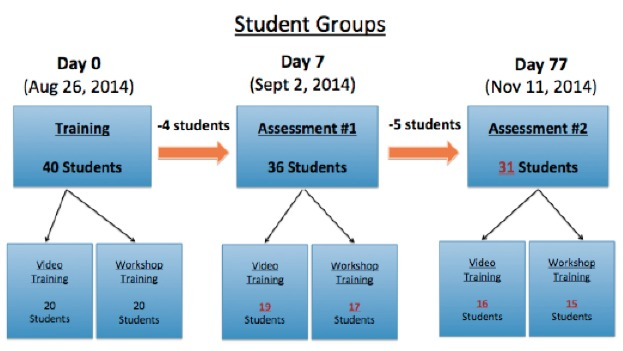
\includegraphics[width=0.8\linewidth]{Pictures/6_studyGroupsExample}
		\caption{Study groups example}
		\label{fig:6_studyGroups}
	\end{minipage}
\end{figure}

\subsection{Procedure}
At first the participant was welcomed and briefed about the idea as well as what she can expect from the study.
Further an introduction about the training method in which she participates was given.
After agreeing to participate on the study she had to confirm a form consent.
Next she had to answer a questionnaire for collecting demographic data and her prior experience with slacklining.
The ISG had to answer one more question about the prior experience with interactive devices (e.g. Kinect, Wii, PlayStation Move, etc.).
%Therefore one can see if a person, which tends to have a better experience with the system during the study, relies on her prior experience with such devices. 
The physical activity level as well as the lateral preference was determined like stated above.

At first the general balance ability of the participant was obtained before pre-measurement to exclude participants with a balance disorder.
Thereby she had to execute a single leg stand for the right and the left foot at first on the ground and then on a towel for a maximum of 10 seconds with 3 trials.
This ensures the participant has no problems with holding her own balance on a stable as well as on a uneven underground.

\todo{as few steps as possible to have a comparison}
After successful accomplishment the actual pre-measurement test was conducted.
It is divided in two parts.
First, a single leg stance for the left and right foot on the slackline with a maximum of 10 seconds.
Second, trying to walk on the entire slackline with the left as well as the right leg as starting point.
For each measurement and leg the participant had to accomplish three trials, which results in an amount of 12 trials.

After finishing the pre-measurements the participant was again shortly introduced about the ongoing procedure.
For all exercises she had to stay on a marked position at the ground, which visualizes the starting point.
Depending on the training method, the introduction, repetitions and time to hold each exercises is provided by the trainer or interactive system.
During the execution either the trainer or the system hints the participant about the correct execution of the exercise.
If an execution was not accurate, she had to repeat it until all repetitions of the exercises are accomplished successfully.
The participant had the possibility to skip the exercise if it was too difficult to accomplish or not appropriately recognised by the system.
During the training she could take breaks if she wanted to.
When accomplishing an exercise set, the participant was asked to rank the exercise she just completed on a scale of 1 (very easy) to 5 (very difficult).
%Therefore the ranking of the participant can be compared with the logged performance data.
%Hereby, it can be shown if the difficulty of the exercise set in each level is increasing and match the users' assumptions. %integrated exercise routine.

After finishing the training part a post-measurement was conducted with the same procedure as in the pre-measurement seen above.

Finally the participant had to answer questions in a semi-structured interview to obtain her opinion on the general training method and application scenarios for exactly this method with the slackline and other sport activities that could fit this method.
The ISG were additionally asked about the user interface of the slackline learning system and their experience with the interaction.
The specific questionnaires and interview questions can be seen in \todo{Appendix}.
%for reviewing and validating performance parameters as well as to detect system failures.

\subsubsection{Apparatus}
Figure \todo{[figure]} shows the setup of the study.
The Kinect was attached on a tripod with a height of \todo{90 cm}.
It is placed in front of a wall, which is used as projector screen.
The camera is faced in the direction of the slackline.
A projector is mounted on the ceiling of the room to project the systems interface on a wall.
The mobile slackline stands, like discussed in Section~\ref{5_1_hardwareComponents}, directly in front of the Kinect.
Marker attached on the slackline provide information for pre- and post-measurements as well as the starting point for the participant to get up the line.
The set up for the human trainer group was the same, but without the projector and the Kinect.
To record the execution a video camera was placed behind the participant to have her actions as well as the interface interaction recorded.
The set up was not changed during the study to have the same condition for every participant.

\todo{[Figure]}


\subsection{Design and independent \& dependent variables}\label{6_variables}
The experiment of the study is a 2 x 2 mixed factorial design, more specifically a 2 levels of group (group: ISG, HTG)  x 2 measurements (time: pre, post).
%Subjects were randomly assigned to a interactive system group (ISG) or a human trainer group (HTG).
Within subject a pre-measurement and post-measurement after the training was conducted.
The measurements are divided into three parts.
First, measuring the time of a single leg stance with the left as well as the right foot on the slackline with a stopwatch by the director of the study.
Second and third, measuring the steps and distance the participant can walk on the slackline with the left and right foot as starting point.
Therefore the slackline was divided into 12 parts with tape marks with a distance of 0.5 meters for each, to be able to measure the distance on the video recording with a certain amount of accuracy.
Three consecutive attempts per side of the foot and method were executed and measured to compare the results.
All pre- and post-measurement were recorded by video.
With the help of these video recordings each trial of the participants were checked twice after the study.

\textbf{Independent variables}
\begin{itemize}
\item Interactive Slackline Group
\item Human Trainer Group
\end{itemize}

\textbf{Dependent variables}
\begin{itemize}
\item Time stood on line with left and right foot
\item As many steps as possible on the line 
\item Walking as far as possible on the line
\end{itemize}

%The time was counted if the balancing leg of the participants leaves the ground and stopped if she gets in contact with the ground with any foot.


%\textbf{Confounding variable}
%\begin{itemize}
%\item Experience with general balance training
%\item Experience with slacklining
%\item General physical activity
%\end{itemize}

%A measurement of the participants' current balance performance was conducted before and after the training to compare the training results and learning progress.  This involves the measurement of how long the participant can stand on the slackline in seconds with her left, right, and with both feet. Further, how many steps were she able to walk on the slackline with the left or right foot for getting up the line. Three attempts per side and method were executed and \todo{the best taken / the average calculated} to compare the results.

% https://explorable.com/pretest-posttest-designs --> The Two Group Control Group Design


\begin{comment}
2 x 2 mixed factorial design
2 within subject --> test
pre-test
post-test

2 between subject --> training
Experiemental group --> ISG
Base line group --> HTG

ODER

3 dependent vs 2 independent variables
\end{comment}
\section{Results and Analysis}\label{6_results}
\begin{comment}
Each calculated variable was averaged across the three consecutive recorded trials.
Further, the data is provided as means with standard deviations.
A two-tailed paired-samples t-test was used to compare the single leg stance (seconds) and walking over the line performance (steps and cm) for the left and right leg before and after training.
For all pre to post variables the difference was calculated to test its normal distribution with the Shapiro-Wilk test and find outliers via boxplots in the dataset.
Because of the small number of subject all tests were verified with the non-parametric Wilcoxon signed ranks test.
An independent-samples t-test was conducted to compare the slackline performance in single leg stance (seconds) and walking over the line (steps and cm) for the left and right leg between the interactive system group and human trainer group.
For all post variables the normal distribution was calculated.
Further, the homogeneity of variance is calculated to meet the requirements of an independent t-test.
Like in the paired-sample t-test a non-parametric Mann-Whitney U test was used to verify the outcome of the independent t-test.
Level of significance was set at $p$ < 0.05.

As non-parametric testing revealed nearly identical results for all conditions as compared to the rANOVA testing procedure, only the parametrical test results will be presented in a uniform manner.
Separate 2 x 2 repeated measures analysis of variance (rANOVAs) with one withing-group (time: Pre vs. Post) and one between-group (group: ISG vs. HTG) factor were calculated to test interaction effects of training, global differences in the dependent variables between pre and post, and possible differences between ISG and HTG.

Two-tailed independent t-test were used to determine possible PRE test differences between the ISG and HTG groups as well as POST test differences.
Further dependent t-tests for paired samples were used to test for differences in dependent variables between PRE and POST.
All outcomes were calculated for each variable separately.
Level of significance was set at p < 0.05.
Effect size was shown by using Cohen's $f$ (partial eta squared) and was defined as small for $f$>0.1, medium for $f$>0.25 and large for $f$>0.4 .
 calculated by the statistics software G*Power 3
\end{comment}

Data are provided as means with standard deviations.
Each calculated variable (for the left and right leg separately in single leg standing time, walked steps over the line, walked distance on the line) was averaged across the three consecutive recorded trials.
Separate 2 (group: ISG and HTG) x 2 (time: PRE and POST) mixed-design repeated measures analysis of variance (rANOVAs) was performed.
To match the requirements of the rANOVA, all parameters were tested on normality with the Shapiro-Wilk test.
Despite walking steps performance in the post measurement for the left and right foot, all data were normally distributed with $p$ > 0.05.
Further, the homogeneity of error variances was assessed by Levene's test with $p$ > 0.05 and the homogeneity of covariances were calculated by Box's test with $p$ > 0.05.
Given these requirements the rANOVA was used for testing interaction effects with sphericity assumed since the group level is < 3, global differences in the dependent variables between PRE and POST, and possible differences between ISG and HTG.
Level of significance was set at $p$ < 0.05.
Effect size was shown by using partial eta squared ($\eta_{p}^{2}$) and was defined as small for $\eta_{p}^{2}$ $\geq$ 0.01, medium for $\eta_{p}^{2}$ $\geq$ 0.06, and large for $\eta_{p}^{2}$ $\geq$ 0.14.

As testing with removed and/or corrected outliers have not shown any essential difference in effects of significance, only the parametrical test results without any removed or corrected data will be shown, to present the results in a uniform manner.
All analyses were performed using SPSS Statistics version 25.

In the following the the requirements and the test results of the mixed rANOVA testing will be reported for each condition separately as well as for the left and right leg.

\subsection{Single Leg Stance Performance}
The homogeneity of error variances was given for the single leg performance for the left and right leg, as assessed by Levene's test with $p$ > 0.05.
There was also homogeneity of covariances, as assessed by Box's test for the left ($p$ = 0.699) and right leg ($p$ = 0.601).

No statistically significant interaction effect between time and group has been found, for the left $F$(1.0, 10.0) = 0.069, p = 0.798, partial $\eta_{p}^{2}$ = 0.007 as well as for the right leg $F$(1.0, 10.0) = 0.004, p = 0.950, partial $\eta_{p}^{2}$ = 0.000.
Since there was no significant interaction effect, the main effects will be reported.

There was no statistically significant main effect within-subjects for time (PRE to POST) for the left leg, $F$(1.0, 10.0) = 3.843, p = 0.078, partial $\eta_{p}^{2}$ = 0.278.
However, a large statistically significant main effect within-subjects for time (PRE to POST) was found for the right leg, $F$(1.0, 10.0) = 15.548, p = 0.003, partial $\eta_{p}^{2}$ = 0.609.

No significant main effect between-subjects for group (ISG to HTG) has been found for the left $F$(1.0, 10.0) = 0.009, p = 0.928, partial $\eta_{p}^{2}$ = 0.001 and right leg, $F$(1.0, 10.0) = 0.008, p = 0.931, partial $\eta_{p}^{2}$ = 0.001.
\begin{figure}[htb]
	\centering
	\begin{minipage}[t]{0.49\linewidth}
		\centering
		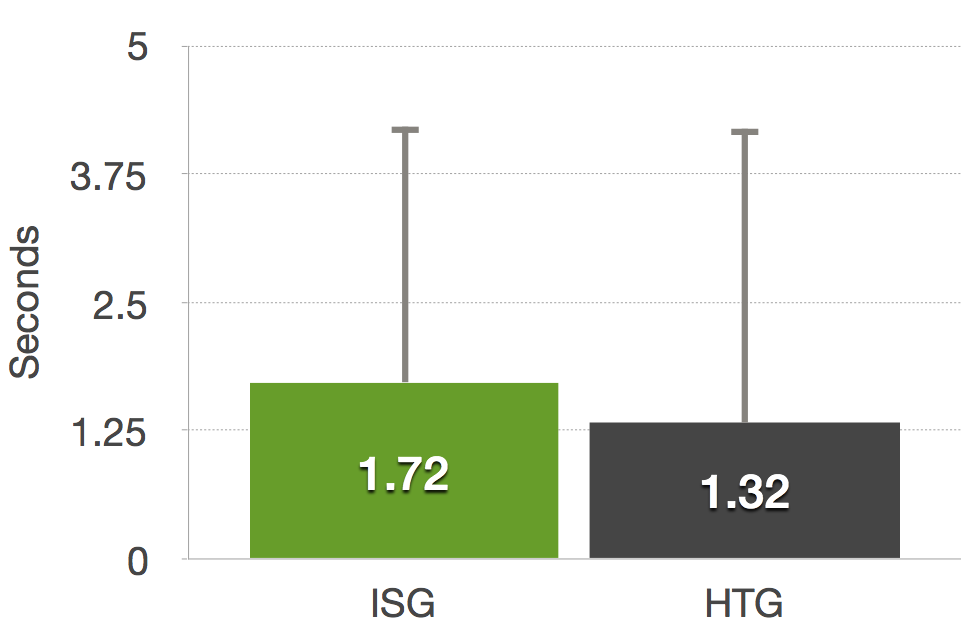
\includegraphics[width=1\linewidth]{Pictures/6_4_DIA_StandLeftDiff}
		\subcaption{Improvement on Standing with Left Leg}
		\label{fig:6_4_standLeftImprovement}
	\end{minipage}
	\hfill
	\begin{minipage}[t]{0.49\linewidth}
		\centering
		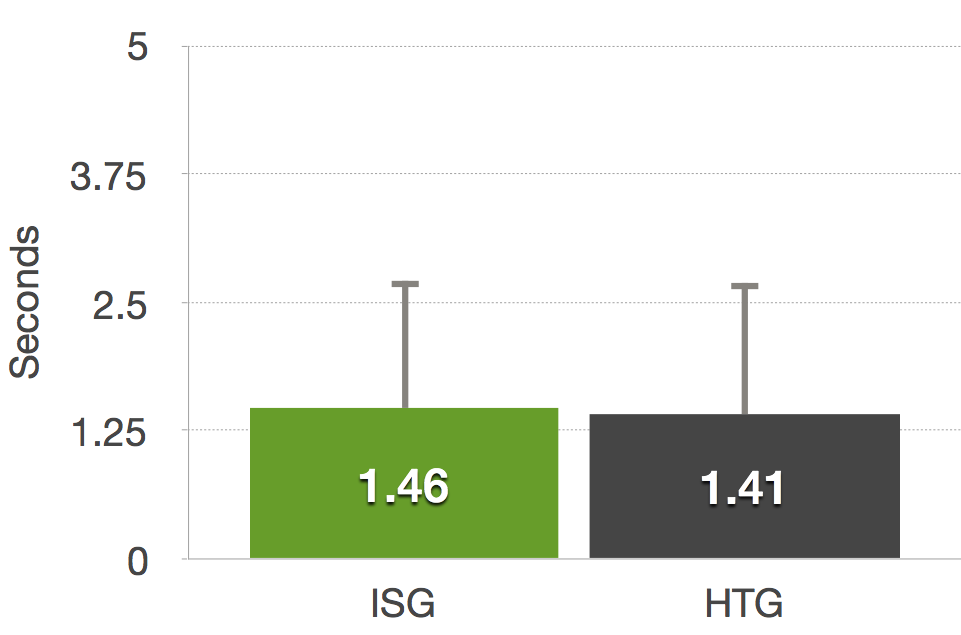
\includegraphics[width=1\linewidth]{Pictures/6_4_DIA_StandRightDiff}
		\subcaption{Improvement on Standing with Right Leg}
		\label{fig:6_4_standRightImprovement}
	\end{minipage}
	\caption{Single Leg Stance Improvement}
	\label{fig:6_4_standImprovement}
\end{figure}


\begin{comment}
\begin{table}[htb]
\centering
\caption{My caption}
\label{my-label}
\resizebox{\textwidth}{!}{%
{\def\arraystretch{1.1}
\begin{tabular}{llrllrlllllll}
\hline
\multicolumn{1}{c}{} & \multicolumn{2}{l}{ISG} &  & \multicolumn{2}{l}{HTG} &  & \multicolumn{6}{l}{Main Effect} \\ \cline{2-3} \cline{5-6} \cline{8-13} 
 & PRE & \multicolumn{1}{l}{POST} &  & PRE & \multicolumn{1}{l}{POST} &  & G x T & $\eta_{p}^{2}$ & T & $\eta_{p}^{2}$ & G & $\eta_{p}^{2}$ \\ \hline
\tab Stand Left (sec) & \multicolumn{1}{r}{4.92 (1.80)} & 6.64 (2.60) & \multicolumn{1}{r}{} & \multicolumn{1}{r}{5.21 (2.25)} & 6.53 (1.65) & \multicolumn{1}{r}{} & p = 0.798 & 0.007 & p = 0.078 & 0.278 & p = 0.928 & 0.001 \\
\tab Stand Right (sec) & \multicolumn{1}{r}{6.44 (2.02)} & 7.90 (2.33) & \multicolumn{1}{r}{} & \multicolumn{1}{r}{6.35 (2.92)} & 7.76 (2.16) & \multicolumn{1}{r}{} & p = 0.950 & 0.000 & \textbf{p = 0.003} & \textbf{0.609} & p = 0.931 & 0.001
\end{tabular}%
}
}
\end{table}
\end{comment}

\subsection{Walked Steps Performance}
The homogeneity of error variances was given for the single leg performance for the left and right leg, as assessed by Levene's test with $p$ > 0.05.
There was also homogeneity of covariances, as assessed by Box's test for the left ($p$ = 0.831) and right leg ($p$ = 0.420).

There was no statistically significant interaction effect between time and group, for the left ($F$(1.0, 10.0) = 0.044, p = 0.838, partial $\eta_{p}^{2}$ = 0.004) as well as for the right leg ($F$(1.0, 10.0) = 1.039, p = 0.332, partial $\eta_{p}^{2}$ = 0.094).
Since no statistical significant interaction effect has been found, the main effects within the tests of within-subject effects will be reported.

There was a large statistically significant main effect within-subjects for time (PRE to POST) for the left leg, ($F$(1.0, 10.0) = 15.868, p = 0.003, partial $\eta_{p}^{2}$ = 0.613) and also for the right leg ($F$(1.0, 10.0) = 12.519, p = 0.037, partial $\eta_{p}^{2}$ = 0.367).

No significant main effect between-subjects for group (ISG to HTG) was found for the left ($F$(1.0, 10.0) = 0.753, p = 0.406, partial $\eta_{p}^{2}$ = 0.070) and right leg ($F$(1.0, 10.0) = 0.351, p = 0.567, partial $\eta_{p}^{2}$ = 0.034).
\begin{figure}[htb]
	\centering
	\begin{minipage}[t]{0.49\linewidth}
		\centering
		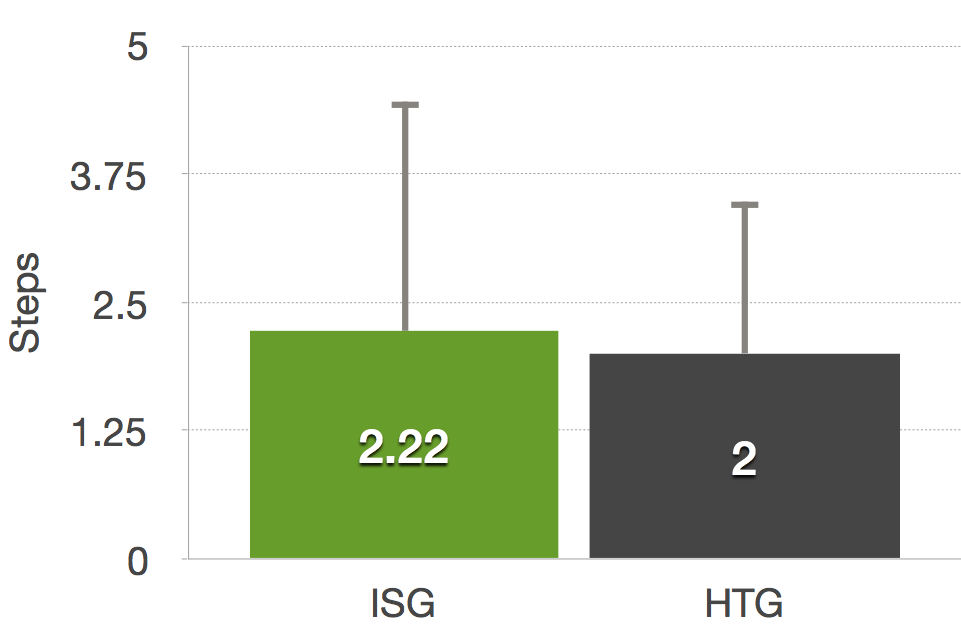
\includegraphics[width=1\linewidth]{Pictures/6_4_DIA_StepsLeftDiff}
		\subcaption{Improvement on Steps with Left Starting Leg}
		\label{fig:6_4_stepsLeftImprovement}
	\end{minipage}
	\hfill
	\begin{minipage}[t]{0.49\linewidth}
		\centering
		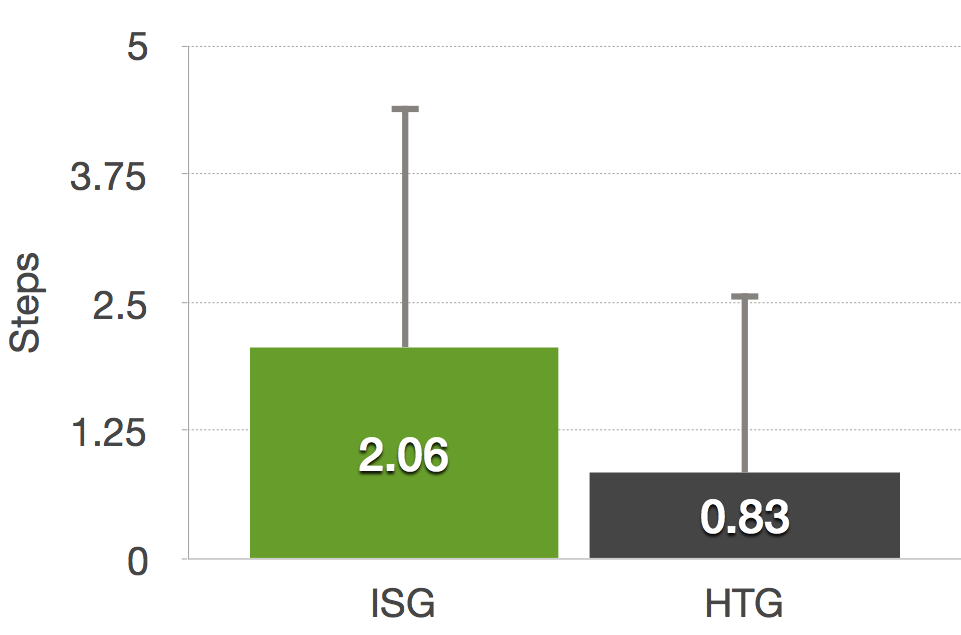
\includegraphics[width=1\linewidth]{Pictures/6_4_DIA_StepsRightDiff}
		\subcaption{Improvement on Steps with Right Starting Leg}
		\label{fig:6_4_stepsRightImprovement}
	\end{minipage}
	\caption{Walked Steps Improvement}
	\label{fig:6_4_stepsImprovement}
\end{figure}

\begin{comment}
\begin{table}[htb]
\centering
\caption{My caption}
\label{my-label}
\resizebox{\textwidth}{!}{%
{\def\arraystretch{1.1}
\begin{tabular}{llrllrlllllll}
\hline
\multicolumn{1}{c}{} & \multicolumn{2}{l}{ISG} &  & \multicolumn{2}{l}{HTG} &  & \multicolumn{6}{l}{Main Effect} \\ \cline{2-3} \cline{5-6} \cline{8-13} 
 & PRE & \multicolumn{1}{l}{POST} &  & PRE & \multicolumn{1}{l}{POST} &  & G x T & $\eta_{p}^{2}$ & T & $\eta_{p}^{2}$ & G & $\eta_{p}^{2}$ \\ \hline
\tab Steps Left & \multicolumn{1}{r}{2.44 (1.26)} & 4.66 (1.53) & \multicolumn{1}{r}{} & \multicolumn{1}{r}{2.06 (1.00)} & 4.06 (1.56) & \multicolumn{1}{r}{} & p = 0.838 & 0.004 & \textbf{p = 0.003} & \textbf{0.613} & p = 0.406 & 0.070 \\
\tab Steps Right & \multicolumn{1}{r}{2.33 (1.05)} & 4.39 (2.00) & \multicolumn{1}{r}{} & \multicolumn{1}{r}{2.61 (1.48)} & 3.44 (0.89) & \multicolumn{1}{r}{} & p = 0.332 & 0.037 & \textbf{p = 0.037} & \textbf{0.367} & p = 0.567 & 0.034
\end{tabular}%
}
}
\end{table}
\end{comment}

\subsection{Walked Distance Performance}
The homogeneity of error variances was given for the single leg performance for the left and right leg, as assessed by Levene's test with $p$ > 0.05.
There was also homogeneity of covariances, as assessed by Box's test for the left ($p$ = 0.712) and right leg ($p$ = 0.193).

There was no statistically significant interaction effect between time and group, for the left ($F$(1.0, 10.0) = 0.006, p = 0.942, partial $\eta_{p}^{2}$ = 0.001) as well as for the right leg ($F$(1.0, 10.0) = 1.235, p = 0.292, partial $\eta_{p}^{2}$ = 0.110).
Since no statistical significant interaction effect has been found, the main effects within the tests of within-subject effects will be reported.

In terms of within-subject time (PRE to POST) a large statistically significant main effect has been found for the left leg ($F$(1.0, 10.0) = 18.563, p = 0.002, partial $\eta_{p}^{2}$ = 0.650) and also for the right leg ($F$(1.0, 10.0) = 7.082, p = 0.024, partial $\eta_{p}^{2}$ = 0.415).

No significant main effect between-subjects for group (ISG to HTG) was found for the left ($F$(1.0, 10.0) = 0.399, p = 0.542, partial $\eta_{p}^{2}$ = 0.038) and right leg ($F$(1.0, 10.0) = 0.145, p = 0.711, partial $\eta_{p}^{2}$ = 0.014).
\begin{figure}[htb]
	\centering
	\begin{minipage}[t]{0.49\linewidth}
		\centering
		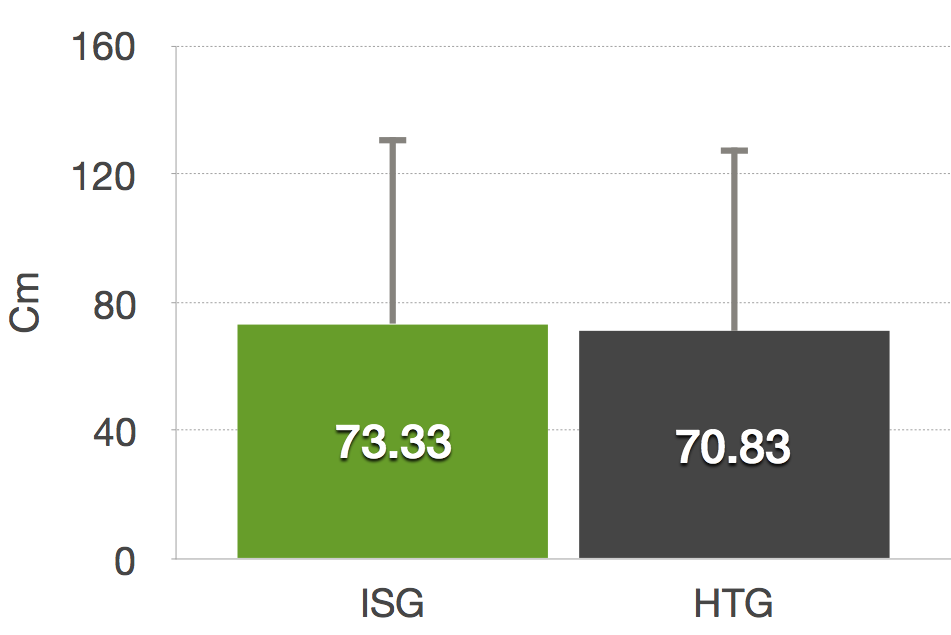
\includegraphics[width=1\linewidth]{Pictures/6_4_DIA_DistanceLeftDiff}
		\subcaption{Improvement on Distance with Left Starting Leg}
		\label{fig:6_4_distanceLeftImprovement}
	\end{minipage}
	\hfill
	\begin{minipage}[t]{0.49\linewidth}
		\centering
		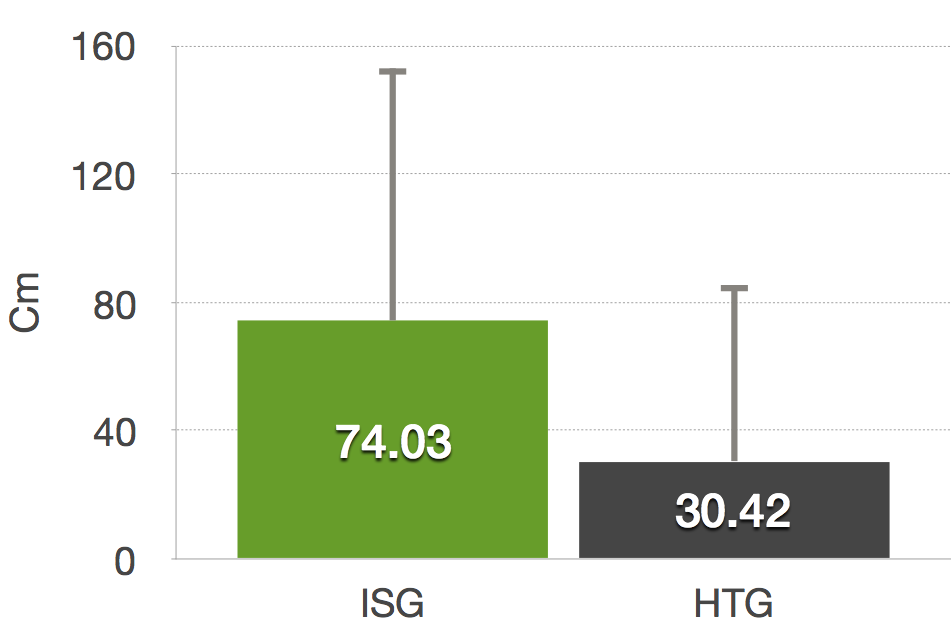
\includegraphics[width=1\linewidth]{Pictures/6_4_DIA_DistanceRightDiff}
		\subcaption{Improvement on Distance with Right Starting Leg}
		\label{fig:6_4_distanceRightImprovement}
	\end{minipage}
	\caption{Walked Distance Improvement}
	\label{fig:6_4_distanceImprovement}
\end{figure}

\begin{comment}
\begin{table}[htb]
\centering
\caption{My caption}
\label{my-label}
\resizebox{\textwidth}{!}{%
{\def\arraystretch{1.1}
\begin{tabular}{llrllrlllllll}
\hline
\multicolumn{1}{c}{} & \multicolumn{2}{l}{ISG} &  & \multicolumn{2}{l}{HTG} &  & \multicolumn{6}{l}{Main Effect} \\ \cline{2-3} \cline{5-6} \cline{8-13} 
 & PRE & \multicolumn{1}{l}{POST} &  & PRE & \multicolumn{1}{l}{POST} &  & G x T & $\eta_{p}^{2}$ & T & $\eta_{p}^{2}$ & G & $\eta_{p}^{2}$ \\ \hline
\tab Distance Left (cm) & \multicolumn{1}{r}{112.92 (35.90)} & 186.25 (43.25) & \multicolumn{1}{r}{} & \multicolumn{1}{r}{101.67 (28.46)} & 172.50 (63.94) & \multicolumn{1}{r}{} & p = 0.942 & 0.001 & \textbf{p = 0.002} & \textbf{0.650} & p = 0.542 & 0.038 \\
\tab Distance Right (cm) & \multicolumn{1}{r}{105.14 (25.30)} & 179.17 (66.65) & \multicolumn{1}{r}{} & \multicolumn{1}{r}{119.17 (56.86)} & 149.58 (36.13) & \multicolumn{1}{r}{} & p = 0.292 & 0.110 & \textbf{p = 0.024} & \textbf{0.415} & p = 0.711 & 0.014 \\ \hline
\end{tabular}%
}
}
\end{table}
\end{comment}

% Please add the following required packages to your document preamble:
% \usepackage{graphicx}
\begin{table}[htb]
\centering
\caption{Means and standard deviation results for single leg stance, walked steps, and walked distance in the interactive system group (ISG) and human trainer group (HTG)}
%\caption{PRE and POST mean and SD values for each condition (ISG and HTG) and measurement variable}
\label{my-label}
\resizebox{\textwidth}{!}{%
{\def\arraystretch{1.1}
\begin{tabular}{lrrrrr}
\hline
\multicolumn{1}{c}{} & \multicolumn{2}{l}{ISG} & \multicolumn{1}{l}{} & \multicolumn{2}{l}{HTG} \\ \cline{2-3} \cline{5-6} 
 & \multicolumn{1}{l}{PRE} & \multicolumn{1}{l}{POST} & \multicolumn{1}{l}{} & \multicolumn{1}{l}{PRE} & \multicolumn{1}{l}{POST} \\ \hline
Stand Left (sec) & 4.92 (1.80) & 6.64 (2.60) &  & 5.21 (2.25) & 6.53 (1.65) \\
Stand Right (sec) & 6.44 (2.02) & 7.90 (2.33) &  & 6.35 (2.92) & 7.76 (2.16) \\
Steps Left & 2.44 (1.26) & 4.66 (1.53) &  & 2.06 (1.00) & 4.06 (1.56) \\
Steps Right & 2.33 (1.05) & 4.39 (2.00) &  & 2.61 (1.48) & 3.44 (0.89) \\
Distance Left (cm) & 112.92 (35.90) & 186.25 (43.25) &  & 101.67 (28.46) & 172.50 (63.94) \\
Distance Right (cm) & 105.14 (25.30) & 179.17 (66.65) &  & 119.17 (56.86) & 149.58 (36.13) \\ \hline
\end{tabular}%
}
}
\end{table}

% Please add the following required packages to your document preamble:
% \usepackage{graphicx}
\begin{table}[htb]
\centering
\caption{Interaction, time, and group effects on single leg stance, walking steps, and walked distance}
%\caption{Significance value and effect sizes ($\eta_{p}^{2}$) for interaction effects, time, and group}
\label{tab:6_4_mainEffects}
\resizebox{\textwidth}{!}{%
{\def\arraystretch{1.1}
\begin{tabular}{lllllll}
\hline
\multicolumn{1}{c}{} & \multicolumn{6}{l}{Main Effect} \\ \cline{2-7} 
 & Group x Time & $\eta_{p}^{2}$ & Time & $\eta_{p}^{2}$ & Group & $\eta_{p}^{2}$ \\ \hline
Stand Left (sec) & p = 0.798 & 0.007 & p = 0.078 & 0.278 & p = 0.928 & 0.001 \\
Stand Right (sec) & p = 0.950 & 0.000 & \textbf{p = 0.003} & \textbf{0.609} & p = 0.931 & 0.001 \\
Steps Left & p = 0.838 & 0.004 & \textbf{p = 0.003} & \textbf{0.613} & p = 0.406 & 0.070 \\
Steps Right & p = 0.332 & 0.037 & \textbf{p = 0.037} & \textbf{0.367} & p = 0.567 & 0.034 \\
Distance Left (cm) & p = 0.942 & 0.001 & \textbf{p = 0.002} & \textbf{0.650} & p = 0.542 & 0.038 \\
Distance Right (cm) & p = 0.292 & 0.110 & \textbf{p = 0.024} & \textbf{0.415} & p = 0.711 & 0.014 \\ \hline
\end{tabular}%
}
}
\end{table}

\subsection{Observations of the User Study}\label{results_interview}
In the pre measurement all participants were very uncontrolled in their body balance and tried to walk fast over the slackline.
After the training in the post measurement, each participant improved to stay and walk with a certain sense of body control on the line.

All participant had fun during the training and enjoyed to play with the system.
They were in general positively surprised by the trackability of the Kinect.

The check list seen in Figure~\ref{fig:6_5_sittingProblems} at the left side above the repetitions and the coloured timer on the mid right side, were mentioned as very useful feedback indicator.

Participants were also motivated to accomplish the current exercises for unlocking the next excises.

Beside these there were also a number of problems that occured.
In the case of general tracking performance with the Kinect there existed problems with the clothing color of a participant.
She showed up with black clothes, and the Kinect had problems to detect her.
This is because black clothing absorb the infrared light of the Kinect, which makes the trackability more difficult \cite{KinectBlackClothing}.

Concerning the exercises during the training problems occurred with the gesture detection while sitting on the slackline for five out of six participants.
Like seen in the user view of Figure~\ref{fig:6_5_sittingProblems}, the leg of the participant was wrongly tracked.
With other participants their leg was often mistaken with the slackline by the Kinect.
All participants of both groups noted also that the sitting exercises are very uncomfortable.
\begin{figure}[htb]
	\centering
	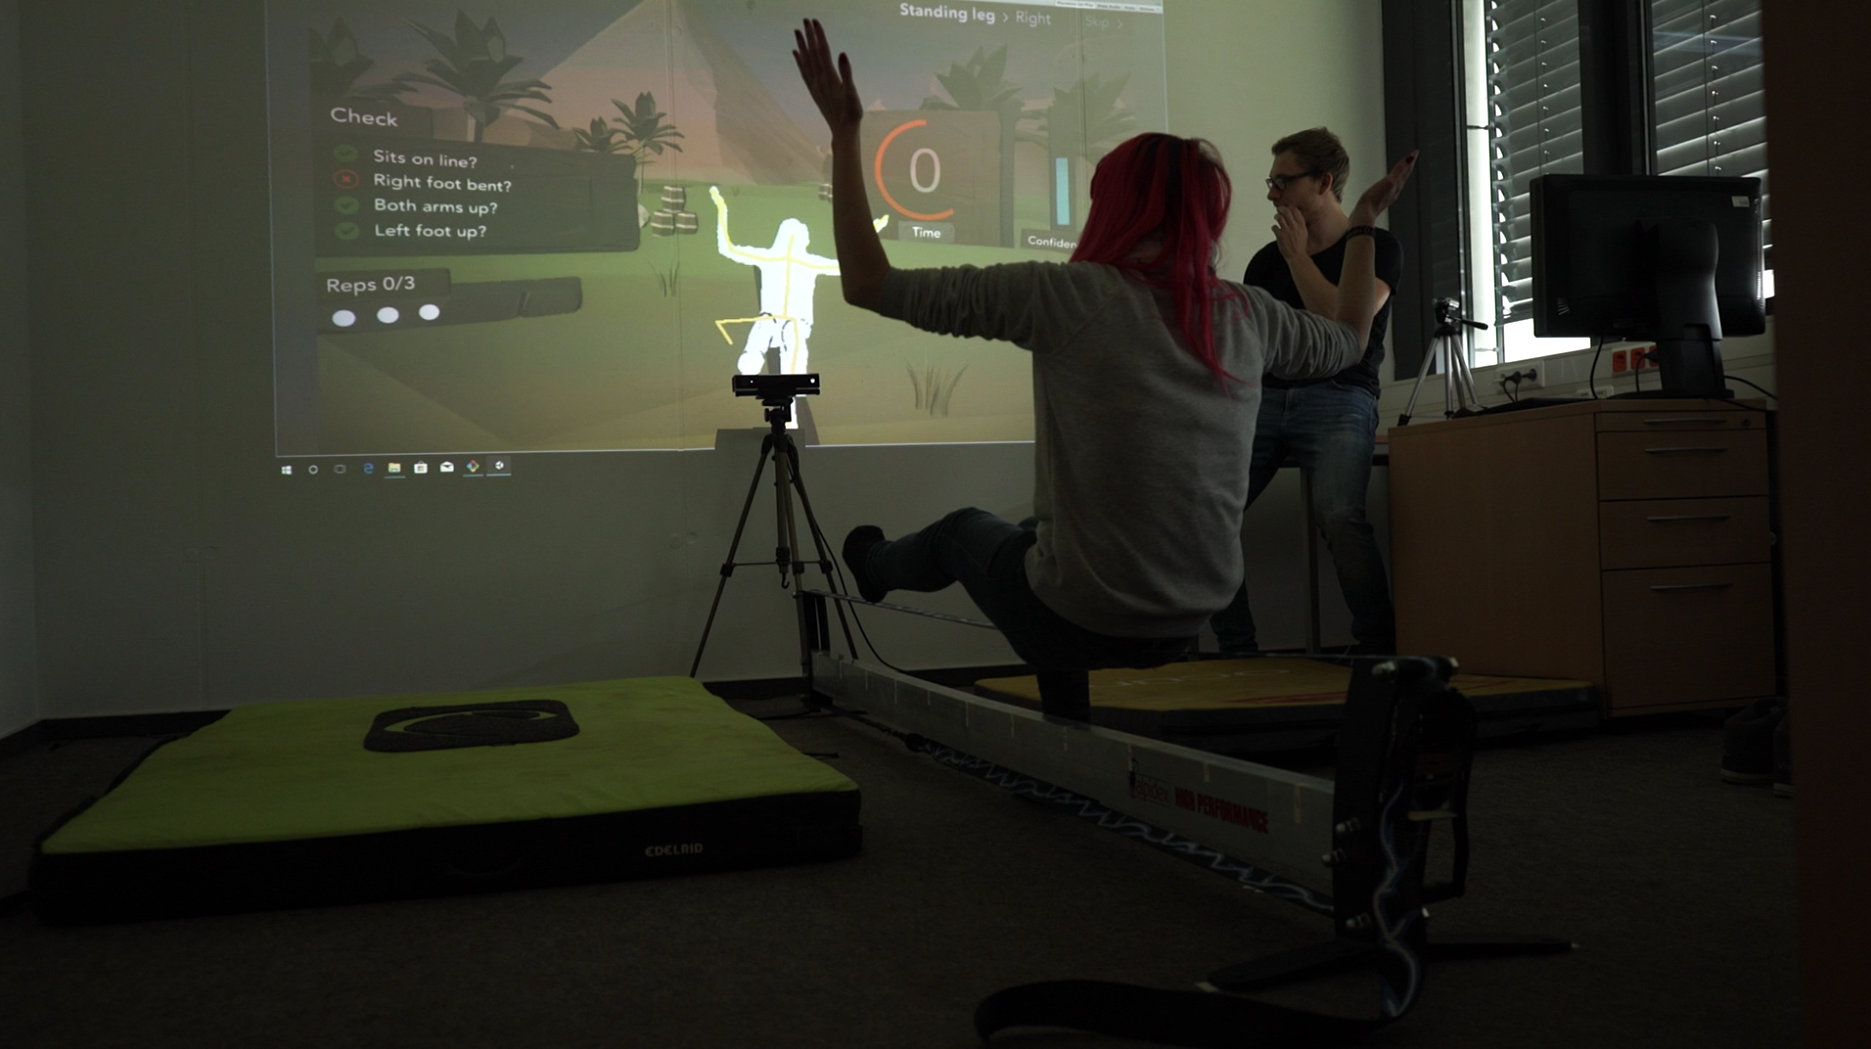
\includegraphics[width=0.88\linewidth]{Pictures/6_5_sitting}
	\caption{The leg of the participant is wrongly tracked by the Kinect, which caused problems for the participant to finish the exercise}
	\label{fig:6_5_sittingProblems}
\end{figure}

The very last exercise resulted also in tracking problems with four out of six participants.
Here, the participants had to walk two steps forward on the slackline and hold the end pose for a half second.

A general problem was going up on the slackline.
If the participant put his outer leg too close to the line while going up, the Kinect did not tracked it appropriately.
The exercise execution was therefore sometimes not successfully counted.

Three participants in the ISG had small problems with the interaction of the system.
Especially with scrolling the exercise list at the beginning, because they didn't know how to interact with it.

\subsection{Rating of Exercise Difficulty}
Participants were asked to rate each exercises after finishing a set of exercises with both legs.
They could choose a difficulty on a scale from 1 (very easy) to 5 (very difficult).
The ratings of all participants were averaged.
Figure \ref{fig:6_4_exerciseDifficulty} shows the ratings of each exercise (blue line) as well as a trendline, which is a linear interpolation of the values (green line).

\begin{figure}[htb]
	\centering
	\begin{minipage}[t]{0.92\linewidth}
		\centering
		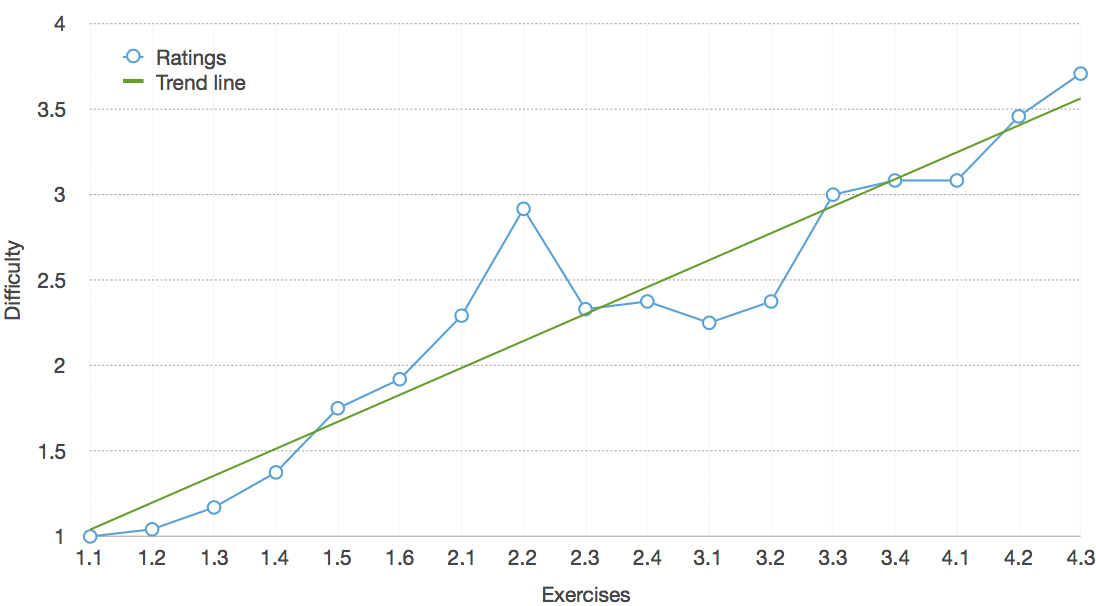
\includegraphics[width=1\linewidth]{Pictures/6_4_DIA_ExerciseDifficulty1}
		\caption{Averaged rating of the exercise difficulty by the participants in blue and the general trend line in green}
		\label{fig:6_4_exerciseDifficulty}
	\end{minipage}
\end{figure}

The exercises of the first level follow a smooth increase in difficulty.
For the second level there is a massive increase in difficulty for the first two exercises.
The ratings for the exercises 2.3, 2.4, 3.1, and 3.2 show comparable difficulty results, since they were the same but exercise 3.1 and 3.2 were different in the time the user has to hold the exercise.
Furthermore, the ratings follow a linear ongoing trend.

\subsection{Semi-Structured Interview}
The general experience with the training method showed similar outcomes for both groups. 
They mentioned a positive learning progress during the training and had a sense of achievement through challenging but practicable exercises.
%Representative participant 10 said: \textit{"The Exercises were well-framed. I felt a learning progress. At the beginning i was not aware of the whole body balance but after the training it could feel how the body balance changed and how I could keep my body in the center of gravity."}

Participant 3 (ISG) mentioned further \textit{"[...]~There is no need to watch YouTube tutorials with such a system. It displays all relevant information and provides appropriate feedback"}.
Participant 4 and 6 (ISG) said a personal trainer could be more helpful due to the fact for giving more specific advises, which the Kinect could not detect.
%answered \textit{"Yes because I have learned something and I do not have to watch YouTube tutorials because it tells me whether I am wrong or not. The user view is also helpful during the exercise execution"}. Participant 4 (ISG) mentioned \textit{"For beginners very well because you can feel and see your own progress through unlocking the exercises. Although a personal trainer could mention things that the Kinect won't detect"}.

The most annoying experience for the ISG was the partially bad gesture recognition of the Kinect and the interaction with it, whereas in the HTG participant 10 mentioned missing exercises for how to get up on the slackline and participant 12 noted especially the uncomfortableness of the sitting on the slackline exercises.

On the other hand, all participants in the ISG liked the environment design, clear description, and especially the looping videos of the exercises as well as the appropriate feedback during the execution.
Participant 6 said further \textit{"I liked the user view because you can see how you act by yourself. It is also positive that I can use the system without any further help."}

Lastly a various amount of application scenarios for the interactive training system were mentioned.
Among others the most stated were physiotherapy, rehabilitation, in general as training for sport activities, gym, and home trainer.


\begin{comment}
%{\def\arraystretch{1.1}

% Please add the following required packages to your document preamble:
% \usepackage{graphicx}
\begin{table}[htb]
\centering
\caption{}
\label{my-label}
\resizebox{\textwidth}{!}{%
{\def\arraystretch{1.1}
\begin{tabular}{lrrrrrrllllll}
\hline
\multicolumn{1}{c}{} & \multicolumn{2}{l}{ISG} & \multicolumn{1}{l}{} & \multicolumn{2}{l}{HTG} & \multicolumn{1}{l}{} & \multicolumn{6}{l}{Main Effect} \\ \cline{2-3} \cline{5-6} \cline{8-13} 
 & \multicolumn{1}{l}{PRE} & \multicolumn{1}{l}{POST} & \multicolumn{1}{l}{} & \multicolumn{1}{l}{PRE} & \multicolumn{1}{l}{POST} & \multicolumn{1}{l}{} & G x T & $\eta_{p}^{2}$ & T & $\eta_{p}^{2}$ & G & $\eta_{p}^{2}$ \\ \hline
\tab Stand Left (sec) & 4.92 (1.80) & 6.64 (2.60) &  & 5.21 (2.25) & 6.53 (1.65) &  & p = 0.798 & 0.007 & p = 0.078 & 0.278 & p = 0.928 & 0.001 \\
\tab Stand Right (sec) & 6.44 (2.02) & 7.90 (2.33) &  & 6.35 (2.92) & 7.76 (2.16) &  & p = 0.950 & 0.000 & \textbf{p = 0.003} & \textbf{0.609} & p = 0.931 & 0.001 \\
\tab Steps Left & 2.44 (1.26) & 4.66 (1.53) &  & 2.06 (1.00) & 4.06 (1.56) &  & p = 0.838 & 0.004 & \textbf{p = 0.003} & \textbf{0.613} & p = 0.406 & 0.070 \\
\tab Steps Right & 2.33 (1.05) & 4.39 (2.00) &  & 2.61 (1.48) & 3.44 (0.89) &  & p = 0.332 & 0.037 & \textbf{p = 0.037} & \textbf{0.367} & p = 0.567 & 0.034 \\
\tab Distance Left (cm) & 112.92 (35.90) & 186.25 (43.25) &  & 101.67 (28.46) & 172.50 (63.94) &  & p = 0.942 & 0.001 & \textbf{p = 0.002} & \textbf{0.650} & p = 0.542 & 0.038 \\
\tab Distance Right (cm) & 105.14 (25.30) & 179.17 (66.65) &  & 119.17 (56.86) & 149.58 (36.13) &  & p = 0.292 & 0.110 & \textbf{p = 0.024} & \textbf{0.415} & p = 0.711 & 0.014 \\ \hline
\end{tabular}%
}
}
\end{table}
\end{comment}

\begin{comment}
\subsection{Two-Tailed Paired-Samples T-Test}
At first will be checked if there are any outliers in the dataset.
Then the results for the normal distribution of each performance condition will be stated since it is a requirement for the two-tailed paired-samples t-test.
After that the results of the significance will be stated.
In the following the outcomes for the single leg stance as well as the steps and distance walked over the slackline will be reported.

\subsubsection{Single Leg Stance Performance}
There were no outliers in the data.
The differences between the pre- and post-scores for the single leg stance were normally distributed, as assessed by the Shapiro-Wilk test for the left leg ($p$ = 0.987) as well as for the right leg ($p$ = 0.203).
There was no difference in single leg stance scores for the left leg before and after the training (t(11) = -2.05, $p$ = 0.065).
The wilcoxon signed ranks test also showed no significant difference (exact significance: $z$ = -1.80, $p$ = 0.077).
Single leg stance score for the right leg was significantly higher after the training (t(11) = -4.14, $p$ = 0.002).
A significant difference was also shown by the wilcoxon signed ranks test (exact significance: $z$ = -2.75, $p$ = 0.003).

\todo{table with means and SD}

\subsubsection{Walked Steps Over the Line Performance}
There were no outliers in the data.
The differences between the pre- and post-scores for the counted steps when walking over the line were normally distributed, as assessed by the Shapiro-Wilk test for the left leg ($p$ = 0.613) as well as for the right leg ($p$ = 0.099).
Steps over the line scores were significantly higher after the training for the left leg, $t$(11) = -4.17, $p$ = 0.002 and for the right leg, $t$(11) = -2.41, $p$ = 0.035.
The wilcoxon signed ranks test also showed significant difference for the left leg (exact significance: $z$ = -2.95, $p$ = 0.001) and for the right leg (exact significance: $z$ = -2.09, $p$ = 0.034).

\todo{table with means and SD}

\subsubsection{Walked Distance Over the Line Performance}
There were no outliers in the data.
The differences between the pre- and post-scores for the distance walked over the line were normally distributed, as assessed by the Shapiro-Wilk test for the left leg ($p$ = 0.358) as well as for the right leg ($p$ = 0.104).
Distance walked over the line scores were significantly higher after the training for the left leg $t$(11) = -4.52, $p$ = 0.001 and for the right leg, $t$(11) = -2.63, $p$ = 0.023.
The wilcoxon signed ranks test also showed significant difference for the left leg (exact significance: $z$ = -2.98, $p$ = 0.001) and for the right leg (exact significance: $z$ = -2.35, $p$ = 0.016).

\todo{table with means and SD}

\subsection{Independent-Samples T-Test}


\subsubsection{Single Leg Stance Performance}

\subsubsection{Walked Steps Over the Line Performance}

\subsubsection{Walked Distance Over the Line Performance}
\end{comment}

\section{\todo{Discussion}}\label{6_discussion}
\begin{comment}
The present study aimed at investigating whether an interactive slackline training system, which 


- results discussion (sport activity people)

- results discussion (lateral preference)

- results discussion (gender)

- observation on study during training

- interview
\end{comment}

\subsubsection{Interaction effects}
No interaction effect for group x time can be shown for any measurement variable for the ISG or the HTG.
This means that no group is better or worse than the other in any measurements.
Therefore the hypothesis that the interactive system shows better results than a human trainer cannot be proven with a statistically significant.
Looking at the figures of the improvements for the group in each measurement \ref{fig:6_4_standImprovement}, \ref{fig:6_4_stepsImprovement}, and \ref{fig:6_4_distanceImprovement}, no real difference can be seen between the groups.
The ISG group is at the most time slightly better in all conditions, which is not sufficient to prove a statistically significance.
A bigger difference can be shown in terms of the right leg side for the walked steps (figure \ref{fig:6_4_stepsRightImprovement}) and walked distance measurements (figure \ref{fig:6_4_distanceRightImprovement}).
It shows that the ISG is approximately 2.5 times better for the right leg.
However the standard deviation of each group is very large, so that it is also not sufficient to have a certain significance.

Since all significance values are larger the defined alpha value of 0.05, the null hypothesis cannot be rejected.
This means that no interaction effect can be found over time from pre to post measurements comparing the groups ISG and HTG and therefore no group is better or worse than the other one.
This can be caused by multiple reasons.
%- Übung zu kurz um unterschied festzustellen

The duration of the training could have been too short to show a statistically significant difference between the groups.
All participants learned just basic techniques of slacklining but no further slackline skill has been trained.
For learning more complex exercises and techniques especially the introduction and feedback given during the execution is very important, since these are key elements of understanding how the exercise works and how to perform it correctly.
Therefore further exercises and further training over a longer time range  could lead to a more specific result, 
%The only difference lied in the effect of how to provide the subject with important information and how to give her feedback about the actual performance.

%- test in zu kurzer zeitspanne um unterschied festzustellen
Second, the participants could have been too exhausted for showing a relevant effect.
Participants trained at least 45 minutes on the slackline.
After this the post measurement has been executed.
Since the training lasted minimum one hour, the measurement results after the training could have been affected by the exhaustion of the participants and therefore not showing there real improvement.
%because of the training could weaken the participant and therefore show not the expected results of an improvement.
%There could be a side effect that participants won't be able to show there real improvements directly after the training due to exhaustion.

%- Unterscheidung zwischen grundlegender balancefähigkeit nicht gemacht somit randomisierte ergebnisse
%alle participants anfgäner auf slackline und keine weiteren ablancetraining bla
% aber nicht nach grundlegenden balanceskill geschaut
% ist bei jedem anders, einer is besser der andere schlechter 
% im test aufgefallen, dass es gute, mittelmäßige und schlechte participants gibt, was sich in der standardabweichung wiederspiegelt
% wennn man die in gruppen einteilen würde bzw auf darauf prüfen würde wie gut die grundlegende balancefähigkeit ist, hätte man ein eingeschränkteres ergebnis, welches die std dev verringert und somit auf signifikanz kommen könnte


Lastly, there was no distinction in general balance skill of the participants.
Subjects were chosen if they had no intermediate slackline experience (i.d. tried slacklining at most two times) or no further balance skill through special sport activities.
The results show a large standard deviation for all variables in the difference of pre to post, because participants improved differently after the training respectively to their pre measurement.
This means that subjects show different general balance characteristics.
Therefore for further studies it is recommended to test on the general balancing skill and characteristic of the participants, to minimize the chance of randomized data because of not qualified participants.

% --> differ the characteristic of balance improvement to reduce randomized data
% --> no distinction in general balance skill
%Third, all participant had to make single leg stance on a common floor and on a rolled towel, which served for validating that no participants has a balance disorder.
%Another reason could be that no grouping of general balance skill has been done.
%In the study only a general distinction of no prior slackline, further balance experience, or balance disorder has been done.

%- dennoch sehr leichter trend für ISG zu verbesserung
However a trend can be observed, that the ISG improved slightly better in numerical average than the HTG.
This could be the case, because the system's gesture recognition is less tolerant about the exercise execution than a human trainer
Whereas a trainer is more tolerant about the users exercise execution, the system has a predefined gesture database, to which the user has to adapt herself.
It leads to more trial executions, because of the strict recognition of the system.

\subsubsection{Time effects}
The time effect seen in table \ref{tab:6_4_mainEffects} in the column \textit{Time} shows whether it differs significantly from pre to post measurement, without considering any group.
This means the time effect is observed for all participants as one entity, like no group would exist.
The results state for all measurement conditions a significant improvement, unless for stand left.
With this it is proven that the used training exercises by both groups are useful and have an effect on the improvement of the participant.

The standing left leg showed no statistically significant result ($p$ = 0.078).
It is more difficult to hold the balance on a weaker leg, because it is less familiar with handling these situations than the primary leg.
Since slacklining is a more complex balance activity, the general balance of the trainee has to be trained with her weaker leg to show an improvement of the slackline specific training.
It can be assumed that less trained legs or participants won't show an improvement as good as participants or legs that have a certain general sense of balance.
Furthermore the physical strain could have exhausted the functionality of the leg, since post results has been measured directly after the training.

In reverse the right leg shows significant results.
For all participants their right leg was the primary leg.
The general balance skill for this leg is given through everyday physical effort and therefore it shows more stable data for balance improvements.

\begin{figure}[htb]
	\centering
	\begin{minipage}[t]{0.32\linewidth}
		\centering
		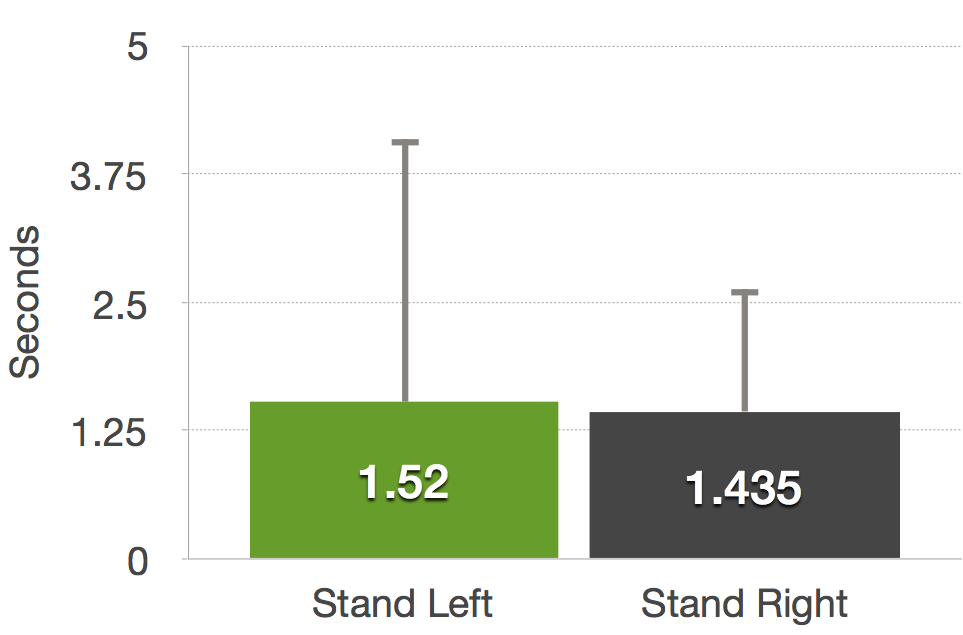
\includegraphics[width=1\linewidth]{Pictures/6_4_DIA_StandAllDiff}
		\subcaption{Improvement on Distance with Left Starting Leg}
		\label{fig:6_4_standAllDiff}
	\end{minipage}
	\hfill
	\begin{minipage}[t]{0.32\linewidth}
		\centering
		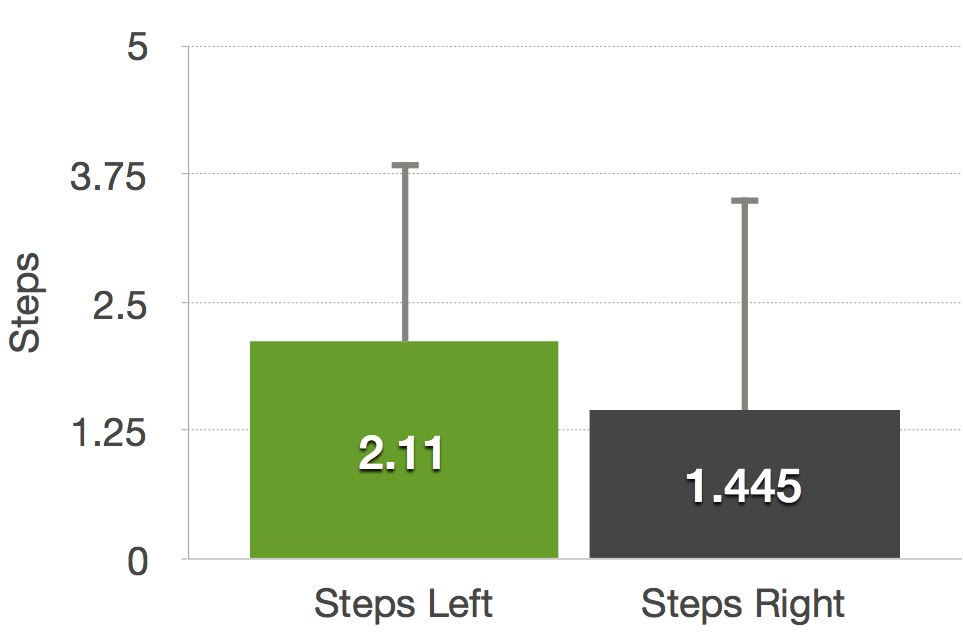
\includegraphics[width=1\linewidth]{Pictures/6_4_DIA_StepsAllDiff}
		\subcaption{Improvement on Distance with Right Starting Leg}
		\label{fig:6_4_stepsAllDiff}
	\end{minipage}
		\hfill
	\begin{minipage}[t]{0.32\linewidth}
		\centering
		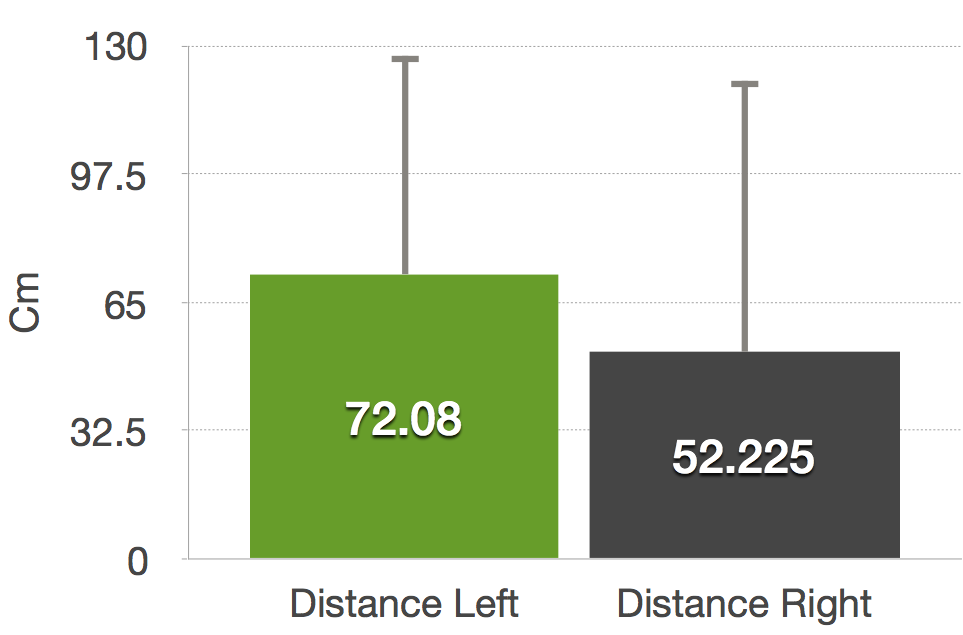
\includegraphics[width=1\linewidth]{Pictures/6_4_DIA_DistanceAllDiff}
		\subcaption{Improvement on Distance with Right Starting Leg}
		\label{fig:6_4_distanceAllDiff}
	\end{minipage}
	\caption{Walked Distance Improvement}
	\label{fig:6_4_distanceImprovement}
\end{figure}

\subsubsection{Group effect}
The main effect for the group is analogue to the previous main effect of the time.
With this, the differences between groups can be calculated, without considering the time.
Looking at table \ref{tab:6_4_mainEffects} in column \textit{Group}, no significant effect can be seen.
This means no group differs from each other.
The diagrams in figure \ref{fig:6_4_mainEffectGroup} show that all results are relatively similar.
Although the ISG is numerically slightly better than the HTG it is not sufficient to have a statistically significance difference.
%no difference calculated
% pre nicht in betracht gezogen
%keine verbesserung der teilnehmer betrachtet
\begin{figure}[htb]
	\centering
	\begin{minipage}[t]{0.40\linewidth}
		\centering
		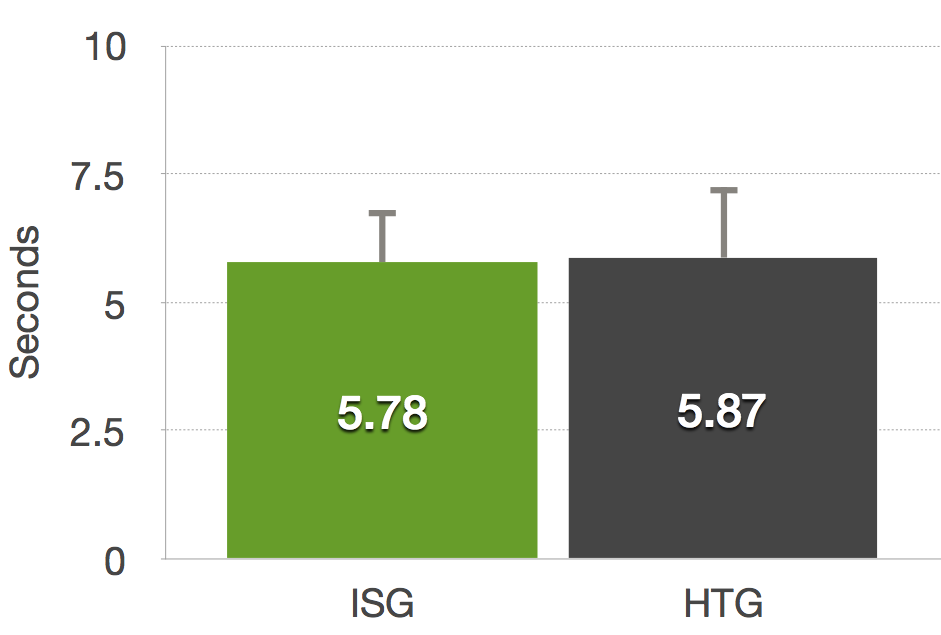
\includegraphics[width=1\linewidth]{Pictures/6_4_DIA_StandLeftGroupEffect}
		\subcaption{Stand Left Results}
		\label{fig:6_4_standLeftGroupEffect}
	\end{minipage}
	\hfill
	\begin{minipage}[t]{0.40\linewidth}
		\centering
		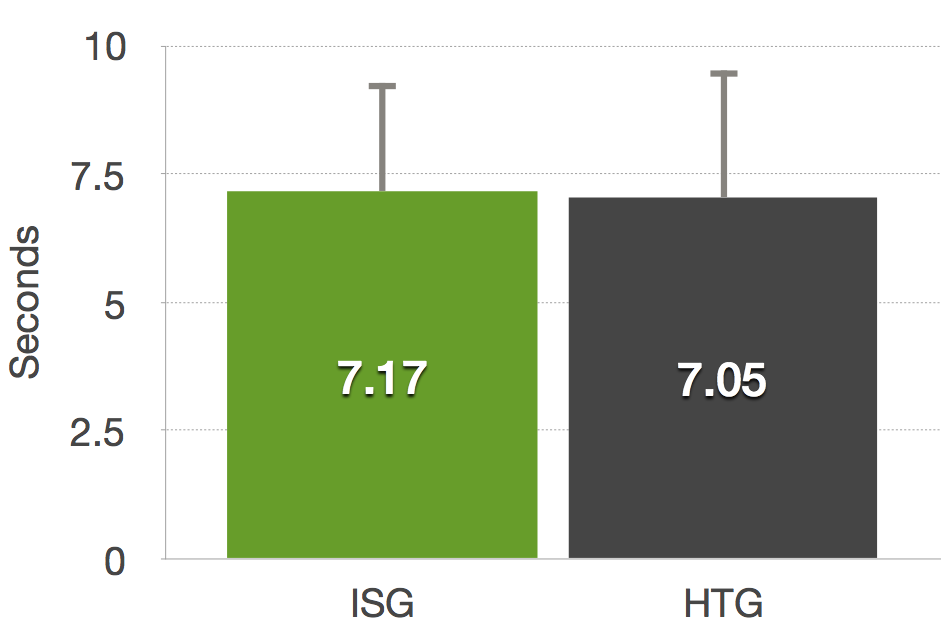
\includegraphics[width=1\linewidth]{Pictures/6_4_DIA_StandRightGroupEffect}
		\subcaption{Stand Right Results}
		\label{fig:6_4_standRightGroupEffect}
	\end{minipage}
	\hfill
	\begin{minipage}[t]{0.40\linewidth}
		\centering
		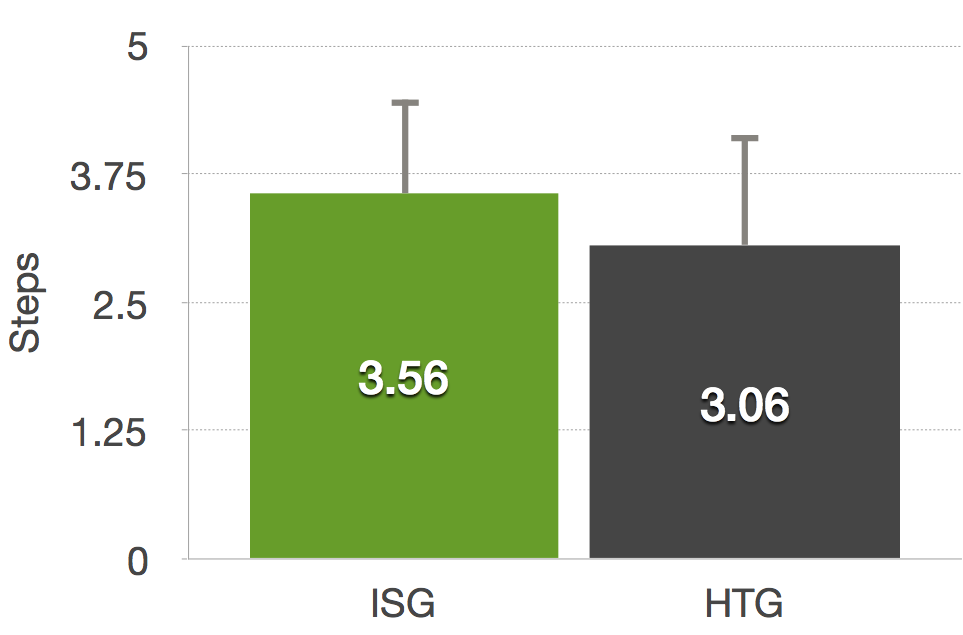
\includegraphics[width=1\linewidth]{Pictures/6_4_DIA_StepsLeftGroupEffect}
		\subcaption{Steps Left Results}
		\label{fig:6_4_stepsLeftGroupEffect}
	\end{minipage}
	\hfill
	\begin{minipage}[t]{0.40\linewidth}
		\centering
		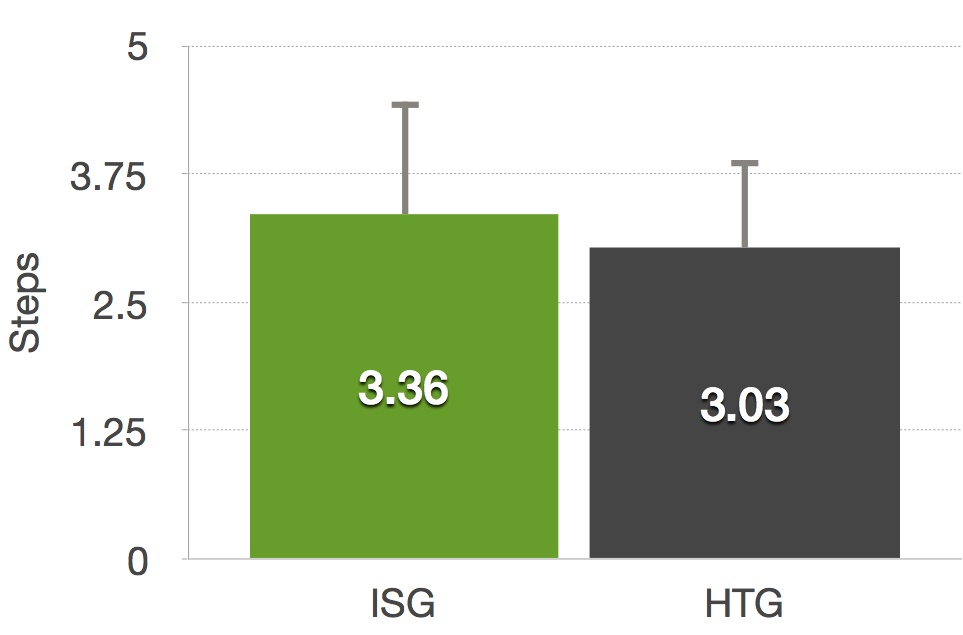
\includegraphics[width=1\linewidth]{Pictures/6_4_DIA_StepsRightGroupEffect}
		\subcaption{Steps Right Results}
		\label{fig:6_4_stepsRightGroupEffect}
	\end{minipage}
	\hfill
	\begin{minipage}[t]{0.40\linewidth}
		\centering
		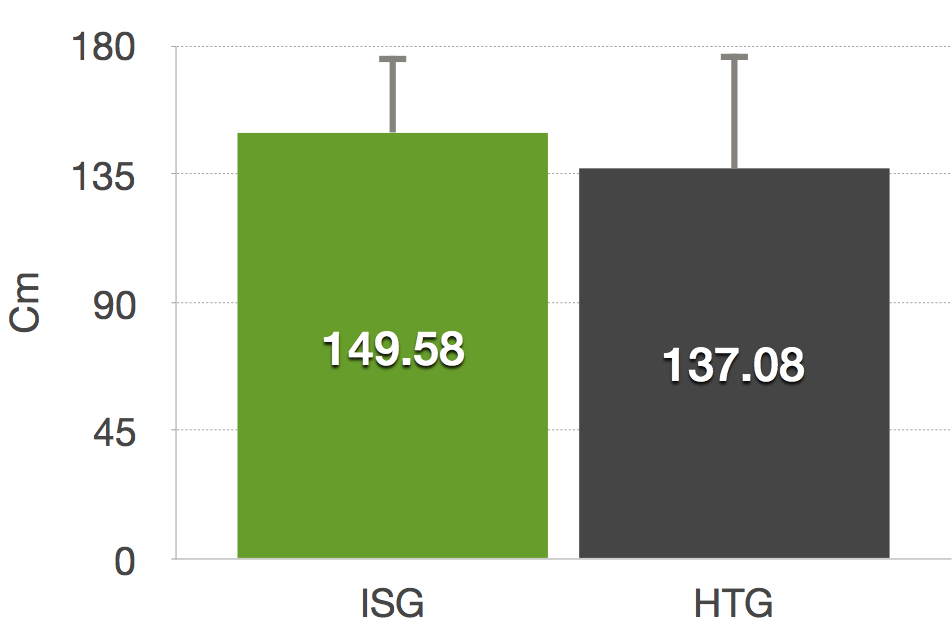
\includegraphics[width=1\linewidth]{Pictures/6_4_DIA_DistanceLeftGroupEffect}
		\subcaption{Distance Left Results}
		\label{fig:6_4_distanceLeftGroupEffect}
	\end{minipage}
	\hfill
	\begin{minipage}[t]{0.40\linewidth}
		\centering
		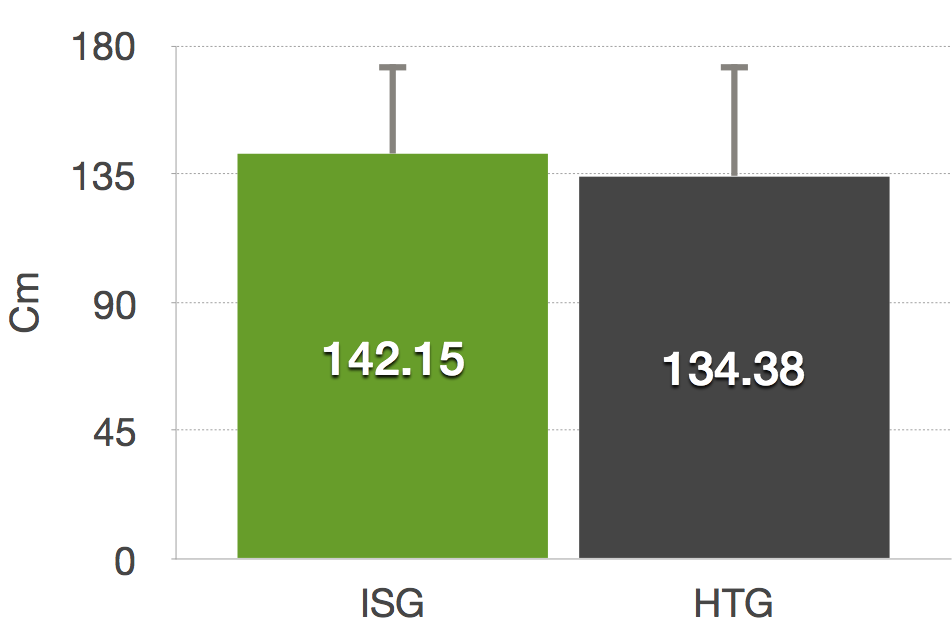
\includegraphics[width=1\linewidth]{Pictures/6_4_DIA_DistanceRightGroupEffect}
		\subcaption{Distance Right Results}
		\label{fig:6_4_distanceRightGroupEffect}
	\end{minipage}
	\caption{Scores for comparing the main effects of the group}
	\label{fig:6_4_mainEffectGroup}
\end{figure}

\subsubsection{Slackline Training Observations}\label{6_4_slacklineObservations}
During the training some observations have been made that would be useful to consider for further practice with the interactive slackline system.

A participant showed up with black pants, which resulted into problems with the Kinect tracking recognition.
This is because some black clothing absorb the infrared light of the Kinect, which makes the trackability more difficult \cite{KinectBlackClothing}.
It would be helpful to indicate participants to not wear any black clothes.

Concerning the exercises there were problems with tracking the participants while sitting on the slackline (Figure \todo{Figure exercise}).
Five out of six participants had problems with this exercise.
Almost all participants out of both groups noted that the sitting exercises are very uncomfortable.
Because of the way the problem exist, this exercise should be eliminated from the exercise list or replaced with exercises to train going up on the slackline.
Like seen in figure \todo{Figure exercise} the leg of the participant was mistaken with the slackline by the Kinect.

The very last exercise resulted also in tracking problems with four out of six participants (Figure \todo{figure}).
Here they had to walk two steps forward on the slackline.
A general problem was the up going on the slackline.
If the leg was too close to the line while going up, the Kinect did not tracked it appropriately.
Both problems could be fixed by tracking the gestures with more persons that execute different variations of a correct exercise execution.

Three participants in the ISG had especially problems with scrolling the exercise list at the beginning because they didn't know how to interact with it.
Adding an introduction on how to scroll a list in the system could be helpful.

\subsubsection{Subjects Rating of exercise difficulty}
Participants were asked to rate exercises after finishing a set of exercises with both legs.
They could choose a difficulty on a scale from 1 (very easy) to 5 (very difficult).
The ratings of all participants were averaged.
Figure \ref{fig:6_4_exerciseDifficulty} shows the ratings of each exercise (blue line) as well as a trendline, which is a linear interpolation of the values (green line).

\begin{figure}[htb]
	\centering
	\begin{minipage}[t]{0.92\linewidth}
		\centering
		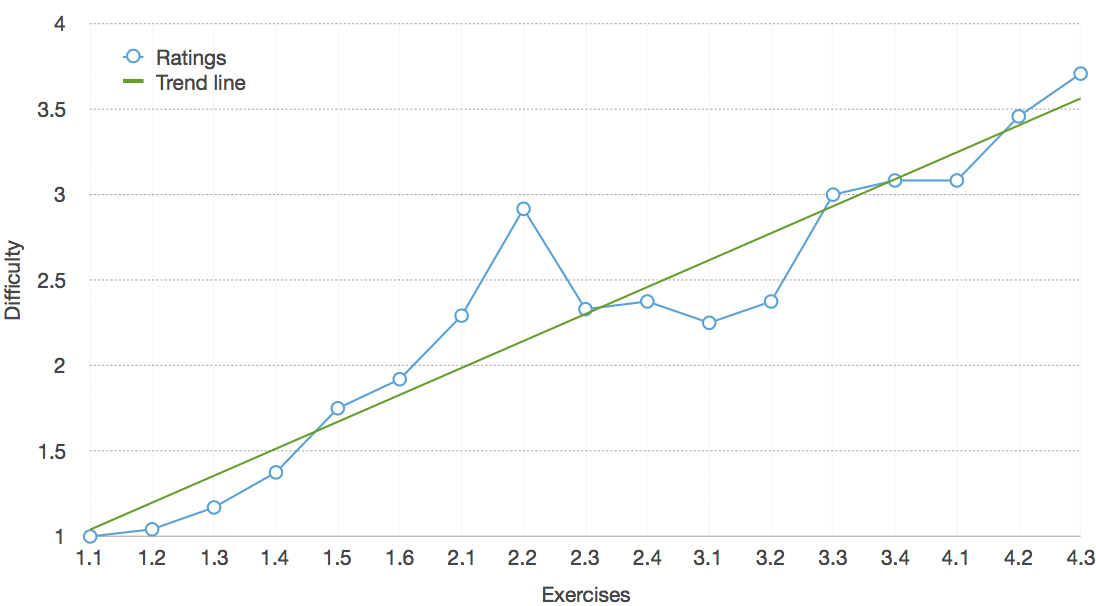
\includegraphics[width=1\linewidth]{Pictures/6_4_DIA_ExerciseDifficulty1}
		\caption{Study groups example}
		\label{fig:6_4_exerciseDifficulty}
	\end{minipage}
\end{figure}

The exercises of the first level follow a smooth increase in difficulty, which matches also the idea of strengthen the general balance skill of the participants and preparing them for standing on a slackline.
For the second level there is a massive increase in difficulty for the first two exercises.
This corresponds also with the observations in section \textit{\nameref{6_4_slacklineObservations}}, where participants claimed that the exercise is very uncomfortable or too difficult for them.
Exercises 2.3, 2.4, 3.1, and 3.2 show similar ratings.
This is because they are all very similar exercises, in which the participant learned to go up on the line.
However the time was increased for exercise 3.1 and 3.2.
Some participants noted that they felt more secure to stand longer on the slackline after doing the short-time exercises.

The ratings follow a linear ongoing trend and therefore verify the appropriate integration of exercises as an entire training model for beginners on a slackline.


\subsubsection{Semi-structured Interview}
The general experience with the training method showed similar outcomes for both groups. 
They felt a positive learning progress during the training and had a sense of achievement through challenging but practicable exercises.
%Representative participant 10 said: \textit{"The Exercises were well-framed. I felt a learning progress. At the beginning i was not aware of the whole body balance but after the training it could feel how the body balance changed and how I could keep my body in the center of gravity."}

Participant 3 (ISG) mentioned further \textit{"[...] There is no need to watch YouTube tutorials with such a system. It displays all relevant information and provides appropriate feedback"}.
Participant 4 and 6 (ISG) said a personal trainer could be more helpful for giving more specific advises that the Kinect could not detect.
%answered \textit{"Yes because I have learned something and I do not have to watch YouTube tutorials because it tells me whether I am wrong or not. The user view is also helpful during the exercise execution"}. Participant 4 (ISG) mentioned \textit{"For beginners very well because you can feel and see your own progress through unlocking the exercises. Although a personal trainer could mention things that the Kinect won't detect"}.

The most annoying experience for the ISG was the partially bad gesture recognition of the Kinect and the interaction with it, whereas in the HTG participant 10 mentioned missing exercises for how to get up on the slackline and participant 12 noted especially the uncomfortableness of the sitting on the slackline exercises.

On the other hand they liked the environment design, clear description and especially the looping videos of the exercises as well as the appropriate feedback during the execution.
Participant 6 mentioend further \textit{"I liked the user view because you can see how you act by yourself. Also I can use the system without any further help"}

Lastly a various amount of application scenarios for the interactive training system were mentioned.
Most mentioned physiotherapy, rehabilitation, in general as training for sport activities, gym, and home trainer.
